\chapter{Roasted Lamb and Potatoes}
\label{ch:lambpotatoes}
\index{meal}
\index{lamb}
\index{Easter}

Family member: Mom \& Dad

\marginnote{
    \textbf{Makes 8+ servings} \\
    Prep time: 45 minutes \\
    Cook time: 1 1/2 - 2 hours \\
    \vspace*{\baselineskip}
    
    1 leg of lamb \\
    Salt \\
    Pepper \\
    3 cloves of garlic, chopped \\
    Olive oil \\
    Oregano \\
    2 lemons, juiced \\
    4 red potatoes, peeled and quartered 
}

\begin{enumerate}
    \item Preheat oven to 350\degree F.
    \item Prepare the leg of lamb: cut the leg into pieces or leave it whole and add it to a large bowl.  Add olive oil, salt, freshly ground pepper and oregano on all its sides, and toss it well. Pierce the leg with a knife and put the pieces of garlic inside. Place the lamb in a large baking dish or roasting pan.
    \item In a bowl, toss the potatoes with olive oil, salt, pepper and oregano and add them to the baking dish.
    \item Pour the lemon juice on the lamb and potatoes, then add 1 cup of water.
    \item Place in the oven uncovered for 1 hour and a half, or until the potatoes are soft and can be pierced easily with a knife. You can add 30 min to make sure there the top of the lamb is crispy!
\end{enumerate}

\begin{figure}
  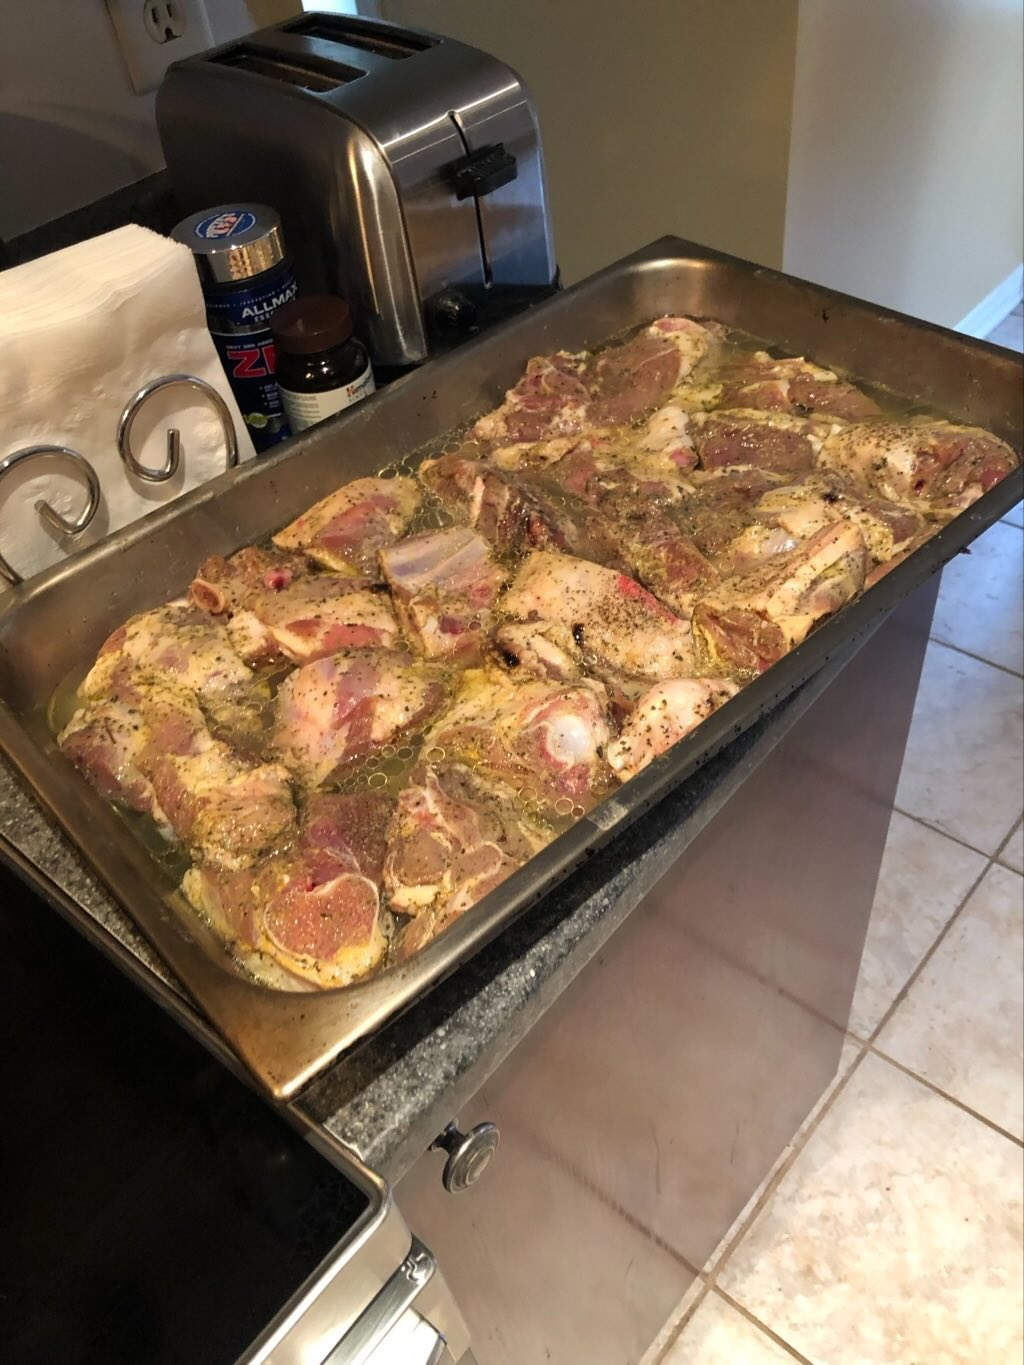
\includegraphics[width=60mm]{monanteras/images/Lamb.jpg}
  \caption{Lamb before putting it in the oven}
\end{figure}
\begin{figure}
  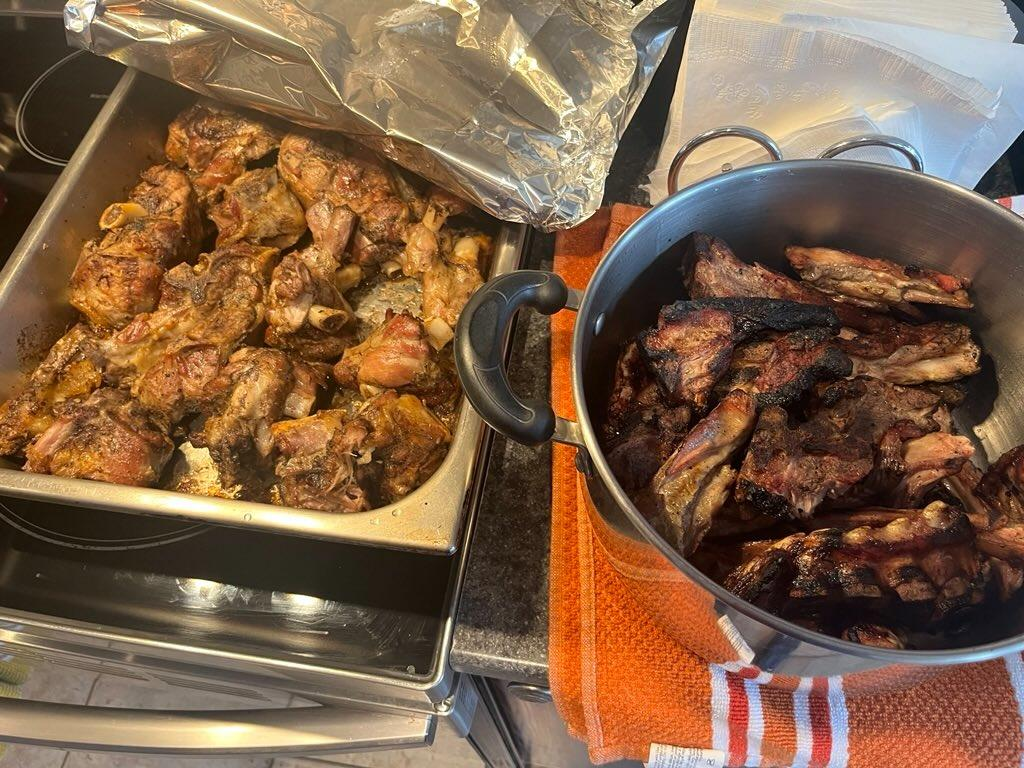
\includegraphics[width=60mm]{monanteras/images/Lamb 2.jpg}
  \caption{Lamb after cooking}
\end{figure}
